% Chapter Template

\chapter{Theoretical Framework} % Main chapter title

\label{Chapter:TheoreticalFramework}

%\subsubsection*{\color{mygray}[Chapter under work]}
% Background and state-of-the-art
% This involves a thorough state-ofthe-art bibliographic review, the building of a formal foundation, the study of related techniques, analysis and awareness of previous works and study of fundamental aspects that can help carry on your research.

\section{Photoresists}
The electronic industry requires sustainable raw material supply for its development \cite{Sutikno2016}. Photoresists are a type of raw material used in microelectronics, which is composed by four main elements: a polymer (resin), a photoactive compound, a solvent, and an additive \cite{Schuster2009}. The additive requires to be with a low molecular weight as it is intended to act as a photosensitive material. Photoresists are used within the manufacturing process of printed circuit boards \cite{Staab2011}. Photoresists are classified into two categories. The resist is defined as positive if the radiation exposed material is soluble in photoresist developer; otherwise, for negative photoresist the exposed material remains to stay in the photoresist surface as it crosslinks upon exposure \cite{Landis2011,Sharma2012}. In the manufacturing process of a semiconductor, the radiation sources which are often used in a lithography process are ultraviolet (UV) and X-ray \cite{Mekaru2015}.

The polymeric material is available on the broad market either in liguid or solid state; \emph{MicroChem Corp.} (Westborough, MA, USA) is the principal provider of SU-8 photoresist. SU-8 and similar photoresists are inexpensive with good adhesion on the semiconductor surface and high sensitivity \cite{Staab2011}. Epoxy resins are copolymer-thermosetting plastics which are normally produced by a chemical reaction process that involves epichlorohydrin and bisphenol-A compound \cite{Singla2010}. A epoxy-based polymer is typically used to produce patterns by lithography with the application of UV radiation. Lithography is a technique to transfer patterns from a mask and then transferred onto the substrate \cite{Landis2011,Xu2014}. SU-8 is a epoxy-based negative photoresist with the advantages of being inexpensive with good mechanical properties, good chemical resistance, and good electrical isolation \cite{Xu2014}. SU-8 photoresists are used in the production processes of MEMS \cite{Zhang2001}. Photoresist-wise, the contrast and quality level of UV radiation lithography is affected by the wavelengths of radiation sources. The higher the sensitivity of the material, the better is the lithography process as it absorbs radiation energy with ease to perform photochemical reactions in forming patterns \cite{Zhang2001}.

In summary, a photoresist is a "epoxy-based resin (polymeric) material which changes its dissolution rate in a liquid solvent, called a developer, under high energy radiation.`` \cite{Landis2011}

\section{Electro-Mechanical Spinning}
Diverse polymer patterning techniques have being develop for the fabrication of nano-fibers, such as arc discharge \cite{Wang2007}, chemical vapor deposition, laser ablation \cite{Ren1998}, and vapor growth \cite{Nadarajah2008}. Nonetheless, those processes are expensive due to either the low product yield or the expensive equipment required. The electrospinning method (invented by Formhals Anton in 1934) can produce fibers with a range of diameters between 10 $n m$ and 10 $\mu m$ \cite{Jayaraman2003,Anton1930} from a polymer solution under the influence of an electrostatic force. The applied electric field and solution conductivity and viscosity is an important parameter the affects the fiber diameter during the spinning along with other parameters such as jet length, solution viscosity surrounding gas, flow rate and the collector geometry \cite{Anton1938,Larrondo1981,Baumgarten1971,Shin2001}.

Even though electrospinning is an old invention \cite{Anton1930}, it is currently a trending topic among researchers \cite{Huang2003,Reneker2008,Schiffman2008}. Some of the reasons electrospinning is to be studied is its potential to fabricate polymer nano-fibers from a variety of polymers. The technique allows the production of thin continuous fibers with ease, with diameters down to 3 $n m$ in some cases, which is something difficult to achieve by other techniques. Furthermore, the basic set-up can be modified with ease to fabricate different fibers with diversified functionalities with different materials. The produced fibers can be aligned or unaligned. Besides, the electrospinning equipment is inexpensive and of small size, compared to the equipment of standard spinning techniques. On the other hand, the understanding of the electrospinning process has improved in the last years \cite{Li2012}. As Reneker and Yarin state: "Electrospinning has rapidly changed fiber making from a capital intensive, large scale process to a low cost, broadly applicable method that manufactures fibers on a laboratory bench, to serve diverse needs ranging from materials science and technology to life sciences and clinical medicine.`` \cite{Reneker2008}

The main components of the electrospinning technique are the fluid control unit (e.g. syringe pump) and a DC power supply. The process also requires a target electrode or combination of electrodes on which the fibers can be collected. Figure \ref{fig:FFES} describes a typical electrospinning set-up. \cite{Li2012}

\begin{figure}[th]
\centering
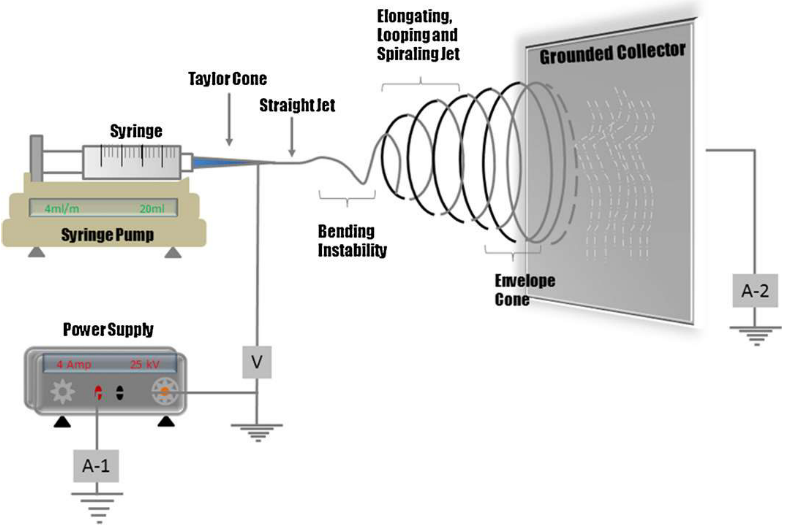
\includegraphics[width=0.75\textwidth]{./Figures/FFES.png}
\decoRule
\caption[Far Field Electrospinning set-up]{Typical far field electrospinning (FFES) set-up \cite{Li2012}.}
\label{fig:FFES}
\end{figure}

Two sub-techniques can be derived from electrospinning depending on the distance between the dispensing electrode and the collector. The process in which the electrospun jet can be controlled near the tip is called NFES or near-field electrospinning. \cite{Cisquella-Serra2019} Moreover, if the distance between the collector and the dispensing needle is farther, the configuration is known as FFES or far-field electrospinning. \cite{Nataraj2012} The difference between NFES and mechano-electrospinning is the presence of a mechanical collector that allows higher precision when patterning. Figure \ref{fig:NFES} shows a typical near field mechano-electospinning apparatus.

\begin{figure}[th]
\centering
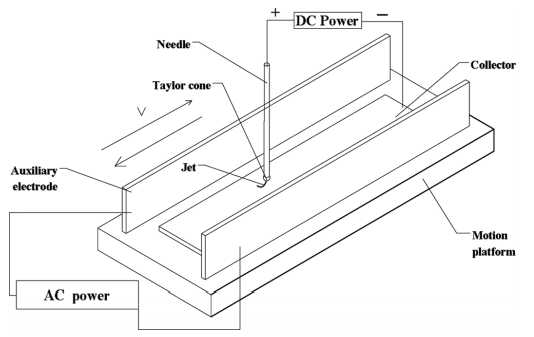
\includegraphics[width=0.75\textwidth]{./Figures/NFES.png}
\decoRule
\caption[Near Field Electrospinning set-up]{Typical near field electrospinning (NFES) set-up \cite{Zhu2016}.}
\label{fig:NFES}
\end{figure}

\section{Pyrolysis}
Pyrolysis is technique that involves heating of biomass in the absence of air or oxygen at a maximum pyrolysis temperature. A small amount of oxygen can burn the structures and make them unusable \cite{Pramanick2018}. Once the maximum pyrolysis temperature is reached, the temperature remains constant to produce solid char, liquids, and non-condensable products. In most cases the liquid product is the main interest of the pyrolysis process, and the properties of the pyrolysis products depend on the maximum pyrolysis temperature and the heating rate \cite{Pramanick2018,Basu2018}.

The heating of large biomass molecules results in decomposition. The pyrolysis decomposition process comprises char, liquids (condensable gases) and non-condensable gases; where the consensable gases may suffer further decomposition into non-condensable gases such as $C O$, $C O_{2}$, $H_{2}$, and $C H_{4}$. Equation \ref{eq:genPyrolysis} is a general representation of the pyrolysis decomposition reaction \cite{Basu2018}.

\begin{equation}
C_{n} H_{m} O_{p} (biomass) \overset{heat}{\rightarrow} \underset{liquid}{\Sigma} C_{x} H_{y} O_{z} + \underset{gas}{\Sigma} C_{a} H_{b} O_{c} + H_{2} O + C (char)
\label{eq:genPyrolysis}
\end{equation}

Pyrolysis yields solid products that are more energy dense than the initial biomass, however the gas and liquid products are less energy dense \cite{Basu2018}. The liquid product of pyrolysis is usually of colour black containing hydrocarbons with a large amount of oxygen and 20\% water. When the liguid product is of interest, a rapid "quenching`` (freeze) is required after pyrolysis to prevent further decomposition or reaction with other substances \cite{Basu2018}. The solid yields of pyrolysis is usually around 85\% carbon with some oxygen, hydrogen and other substances that are present within the initial biomass \cite{Basu2018}. The biomass decomposition by pyrolysis produces non-condensable and condensable gases. The vapors (condensable gases) add up to the liquid yield of pyrolysis which is generated upon cooling. The gases (non-condensable gases) are comprised by ethylene, ethane, methane, carbon monoxide and carbon dioxide \cite{Basu2018}.

\section{Carbon nano-wire}
Carbon nano-wires (CMWs) are known as long, thin strings with diameters between 10 and 1 thousand $n m$; composed mostly by carbon atoms aligned parallel to the long axis of the fiber \cite{Nataraj2012}. Carbon nano-wires are different from carbon nano-tubes, as CMWs are not composed by graphene sheets in cylindrical form \cite{Nataraj2012}. Carbon nano-wires are typically fabricated by electrospinning and pyrolysis/carbonization as the main processes. During the fabrication process, the polymer molecules are to be crosslinked to prevent melting during the subsequent pyrolysis. The carbonization step removes non-carbonized components in form of condensable and incondensable gases \cite{Basu2018} to then yield carbon structures of about 50\% to 75\% of the mass of the original polymeric structure \cite{Nataraj2012}.

\section{Polymer Solutions}
Polymer solutions display viscoelastic properties that provide unique properties due to their macromolecules. their chains are long and entangled. When a shear force is applied, the solution creates a large interaction between the molecules, hence the viscosity depends not only on temperature and shear, but also molecular weight distribution and concentration. The solvent also affects the viscosity \cite{Flores2017, Huang2003, Baumgarten1971}.

\begin{figure}[th]
\centering
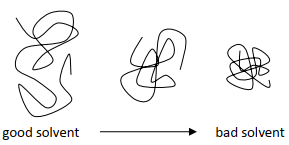
\includegraphics[width=0.50\textwidth]{./Figures/goodbadsolvent.png}
\decoRule
\caption[Effects in polymer chains dimensions due to solvent quality]{Effects in polymer chains dimensions due to solvent quality \cite{Flores2017}}
\label{fig:goodbadsolvent}
\end{figure}

Figure \ref{fig:goodbadsolvent} shows how the quality of a solvent affects the polymer distribution within the solution. Moreover the prsence of electrolites also modify the structure of the polymer threads. In non-ionic solvents, the charges are distributed along the chains and their own repulsion stretches the polimer threads into a more aligned configuration when an electrolyte is added, as detailed in Figure \ref{fig:electrolyteConcentration}.

\begin{figure}[th]
\centering
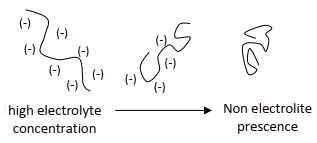
\includegraphics[width=0.50\textwidth]{./Figures/electrolyteConcentration.png}
\decoRule
\caption[Effects of electrolyte in polymer chain dimensions]{Effects of electrolyte in polymer chain dimensions \cite{Flores2017}}
\label{fig:electrolyteConcentration}
\end{figure}

\section{Rheometry}
Rheometry is the measuring technology used to determine rheological data. There are different measuring systems, instruments and analysis methods. Both, liquids and solid  can be investigated using rotational and oscillatory rheometers. Rotational tests are performed to characterize viscous behavior. In order to evaluate viscoelastic behavior, creep tests, relaxation tests and oscillatory tests are performed \cite{Flores2017}.

\subsection{Amplitude Sweep}
An amplitude sweep is a typical test used to characterize the behavior of a polymer
solution or polymer melt. In this basic test a constant angular frequency is applied along with an increasing or decreasing deformation or strain, see Figure \ref{fig:ampSweep} a). The obtained results are the storage and loss moduli, $G'$ and $G''$ respectively, along the values of percentage of strain applied. The amplitude is the maximum of the oscillatory motion. Normally at low frequencies the viscoelastic material presents a linear behavior, this is when the viscoelastic properties are independent of the strain or stress imposed due to the structure of the material stays undisturbed. Nevertheless, as the amplitude is increased at some at some point this linear trend changes suddenly. Once this critical amplitude value is reached the material becomes more elastic or viscous depending on the solution initial state, see Figure \ref{fig:ampSweep} b) \cite{Flores2017}.

\begin{figure}[th]
\centering
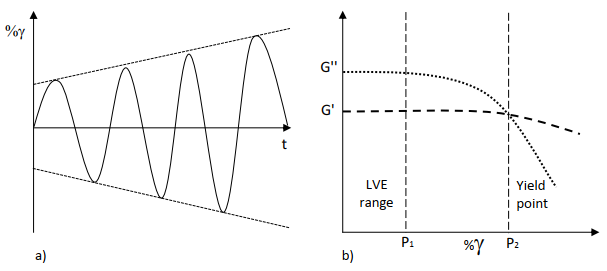
\includegraphics[width=0.75\textwidth]{./Figures/ampSweep.png}
\decoRule
\caption[Amplitude Sweep]{a) Imposed amplitude along time with constant frequency. b) Results for an amplitude sweep \cite{Flores2017}}
\label{fig:ampSweep}
\end{figure}

\subsection{Frequency Sweep}
A frequency sweep, is a common oscillatory test useful to understand the rheological behavior of fluids as it measures the viscoelastic properties. This measurement is considered a viscoelastic spectrum, in general, the shorter the timescale the more elastic the material behaves. These results are related to the molecular structure of the sample. Figure \ref{fig:freqSweep} shows a typical data for a polymer melt where different regions are observed. Frequency sweep measurements also allow the estimation of the molecular weight distribution characteristics such as entanglement density and process-ability \cite{Flores2017}. 

\begin{figure}[th]
\centering
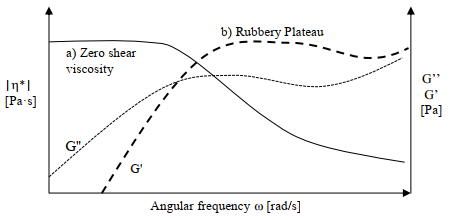
\includegraphics[width=0.75\textwidth]{./Figures/freqSweep.png}
\decoRule
\caption[Frequency Sweep]{Typical results for a frequency sweep. \cite{Flores2017}}
\label{fig:freqSweep}
\end{figure}

\subsection{Flow Curve}
The viscosity is measured as a function of the shear rate in a rotational rheometer with different geometries according to the sample. Normally three types of behaviours can be characterized in flow curve measurements: a) ideal viscous, b) shear thinning and c) shear thickening. Figure \ref{fig:flowCurve} shows three different materials and their response to an imposed shear rate \cite{Flores2017}.

\begin{figure}[th]
\centering
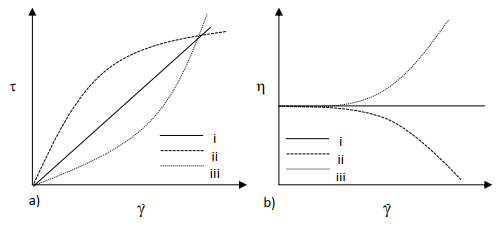
\includegraphics[width=0.75\textwidth]{./Figures/flowCurve.png}
\decoRule
\caption[Flow Curves]{a) Flow curve stress vs stress. b) Flow curve strain vs shear viscosity. Both figures for i Newtonian fluid, ii Shear thinning fluid, iii Shear thickening fluid. \cite{Flores2017}}
\label{fig:flowCurve}
\end{figure}

\section{Preliminary Experiments}


To verify Flores' work \cite{Flores2017}, a series of rheological measurements have been executed. Since one purpose of the proposed dissertation is to replace

%----------------------------------------------------------------------------------------
%	SECTION 1
%----------------------------------------------------------------------------------------



%-----------------------------------
%	SUBSECTION 1
%-----------------------------------


